\section{Valve Closing Model} \label{sec: Prog}

A diagram showing the full arrangement of the pilot-operated pressure relief valve to be considered can be seen in \cref{fig: Diagram}. As the chatter instability was mainly observed during the closing of the main valve~\cite{Allison2015TestingValves}, perhaps the simplest model considers the situation when the main valve is open and the pilot valve has just closed. The pilot valve dynamics can be neglected, as it remains shut. Additionally, the upstream pipework is initially neglected. A zero length pipe ($L=0$) can be considered, meaning the main valve is directly connected to the tank. 

%\begin{figure}[ht]
\begin{figure}[ht]
    % COMPLETE DIAGRAM
    \begin{subfigure}{0.6\textwidth}
    \centering
    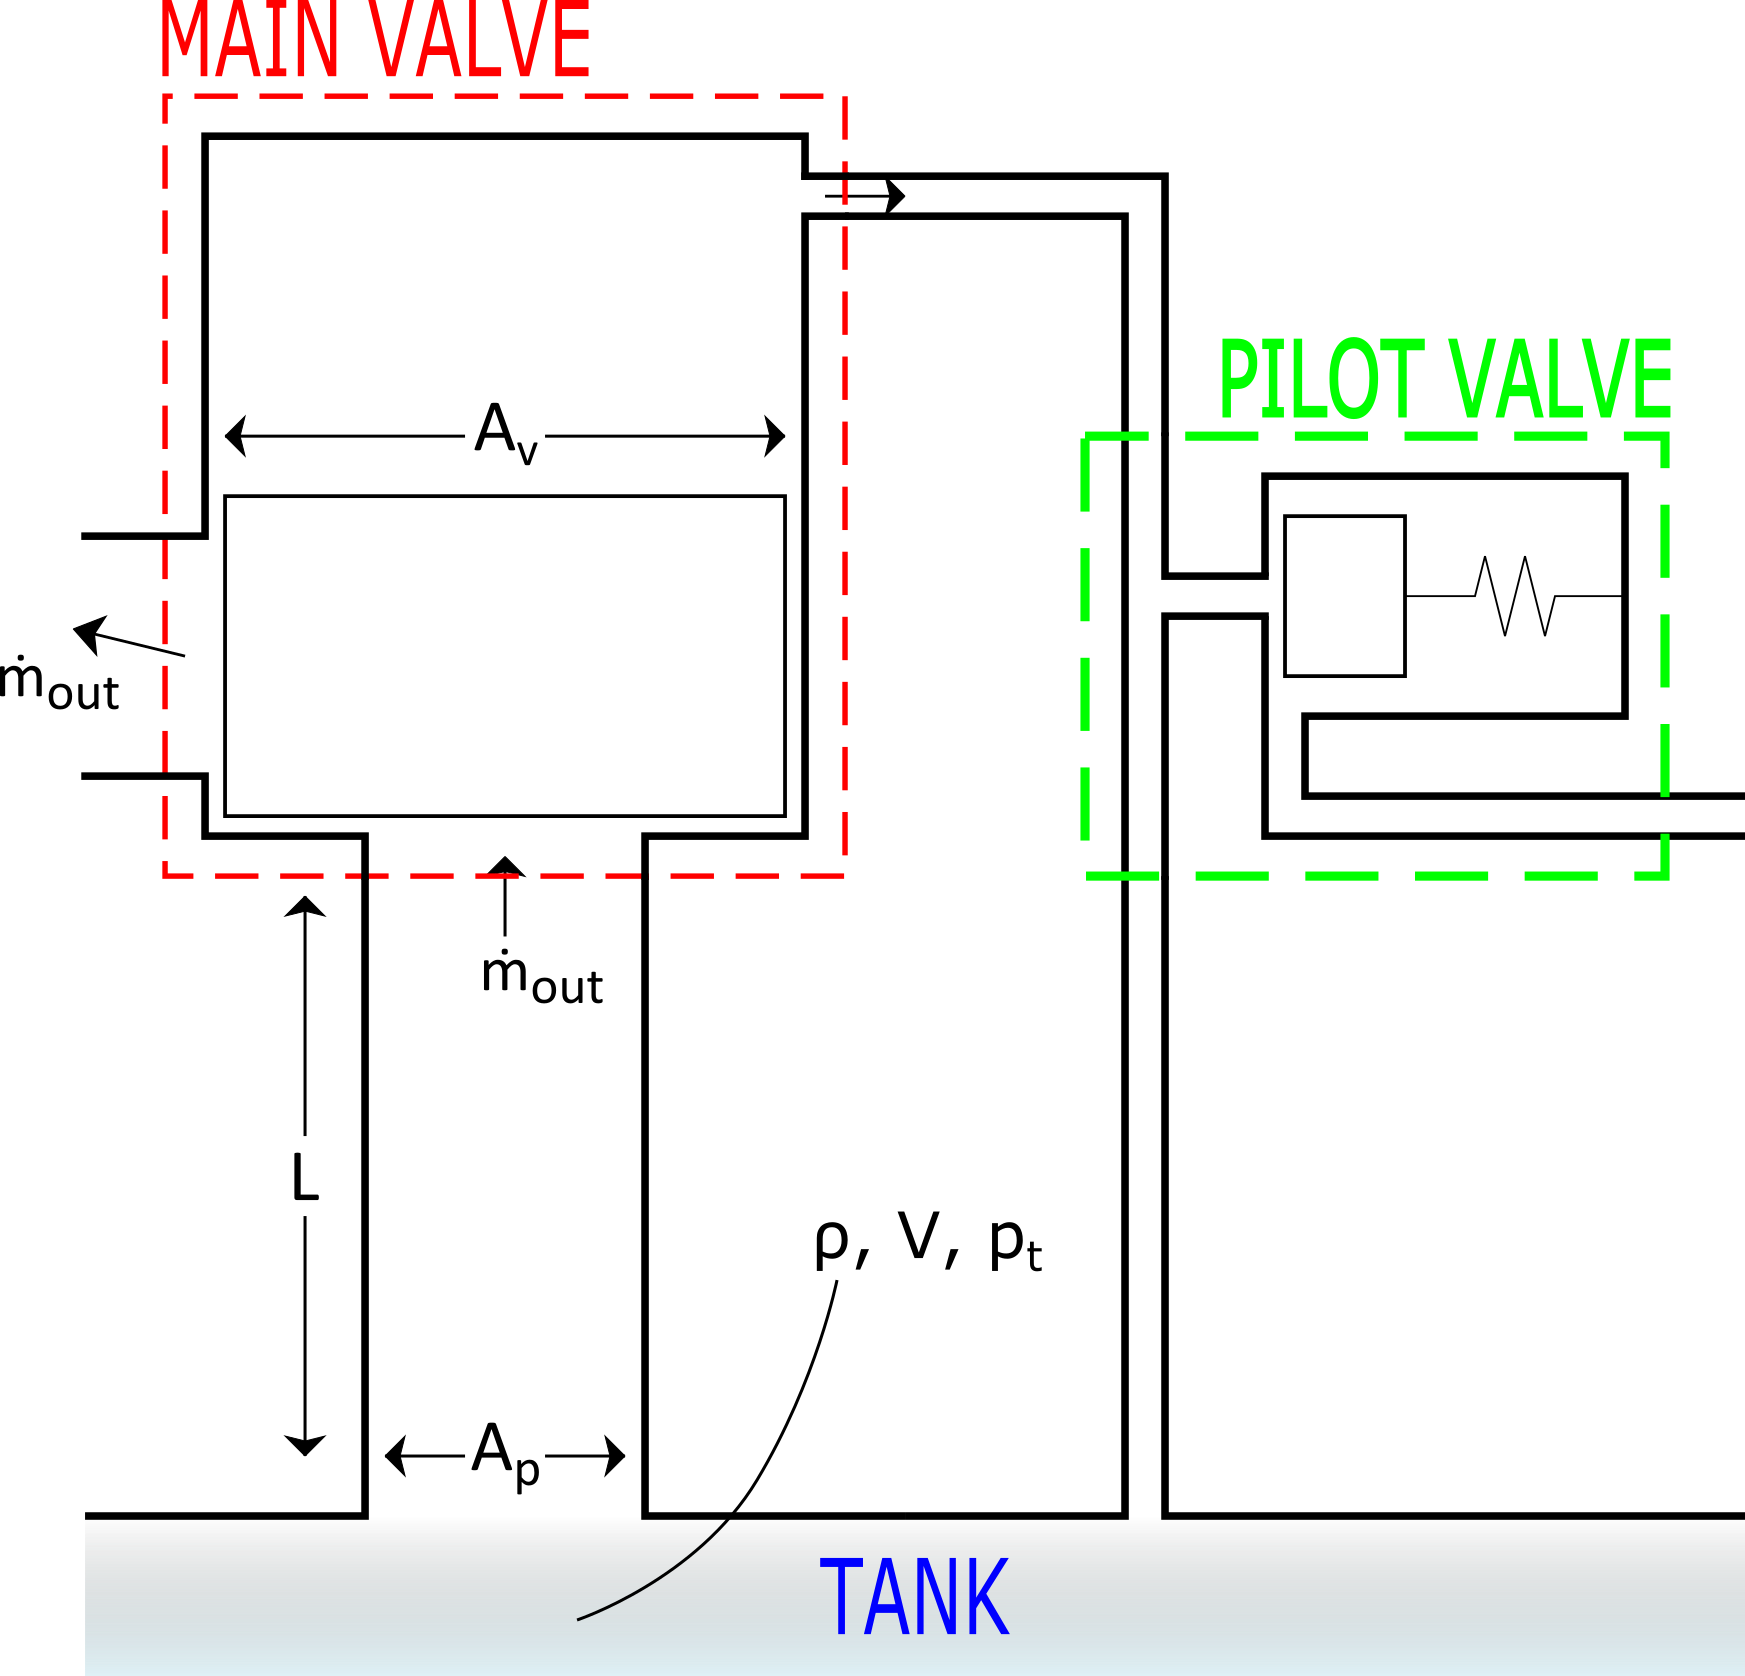
\includegraphics[width=\textwidth]{Diagrams/Diagram.png}
    \caption{Complete valve}
    \label{fig: DiagramComp}
    \end{subfigure}
    \hfill
    % Separate valve figures
    \begin{minipage}{0.3\textwidth}
        % MAIN DIAGRAM
        \begin{subfigure}{\textwidth}
        \centering
        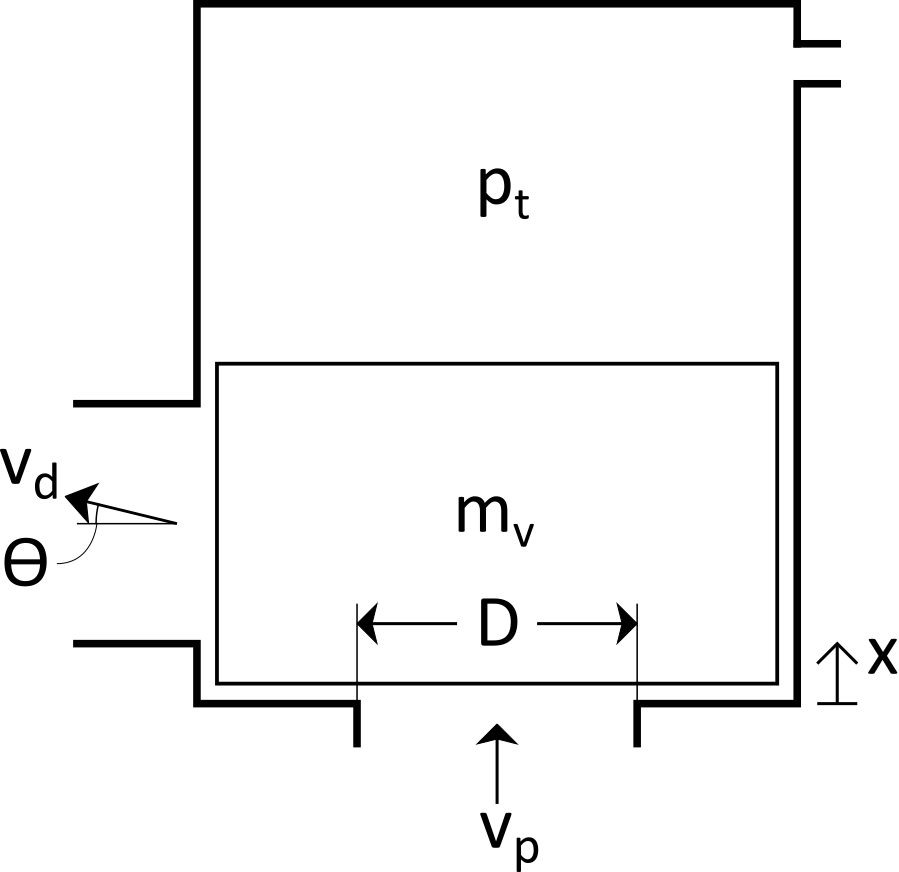
\includegraphics[width=\textwidth]{Diagrams/Diagram-Main.png}
        \caption{Main Valve}
        \label{fig: DiagramMain}
        \end{subfigure}
        % PILOT DIAGRAM
        \begin{subfigure}{\textwidth}
        \centering
        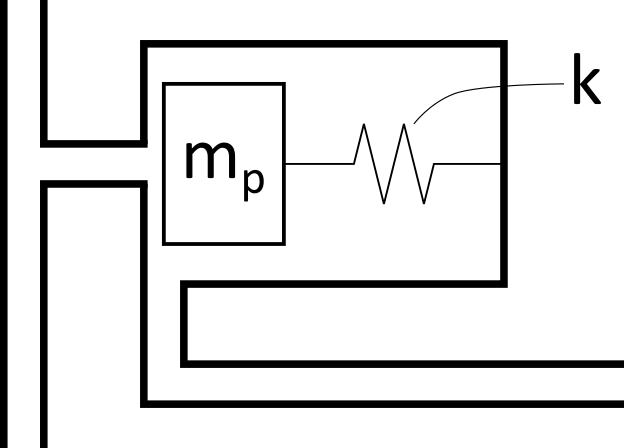
\includegraphics[width=\textwidth]{Diagrams/Diagram-Pilot.png}
        \caption{Pilot Valve}
        \label{fig: DiagramPilot}
        \end{subfigure}
    \end{minipage}
    % Figure caption and label
    \caption{Diagram of pilot-operated pressure relief valve}
    \label{fig: Diagram}
\end{figure}
%\end{figure}

Within the main valve, the fluid can be considered to act on the piston in three ways. The pressure above the piston, in the volume known as the dome, exerts a pressure force across the piston area, $A_v$. This dome pressure is assumed to be equal to the tank pressure. The jet of fluid from the inlet piping exerts a pressure and undergoes change of momentum due to the valve. For simplicity, the jet of fluid is assumed to act over an area equal to the piping cross-sectional area, $A_p$. The force exerted on the valve is equal to the momentum change exerted by the valve to cause the fluid to change flow direction. Combining all of these forces, the motion of the main valve piston can be described by
%\subsection{Valve closing}

\begin{equation} \label{eq: Newton}
    m_v \ddot{x} + c_v \dot{x} = - A_v p_t + A_p p_p + \dot{m}_{out} \left( v_p - v_d \sin(\theta) \right) \, .
\end{equation}

Here, $m_v$ is the valve piston mass, $c_v$ is the valve damping, $p_p$ is the pressure at the end of the pipe, and $\theta$ is the discharge angle. $v_p$ is the velocity of the fluid between the main valve and tank through the orifice or zero length pipe, which will now simply be referred to as the pipe velocity.

%\newpage
Clearly, the properties which depend on fluid dynamics must be expressed in terms of the piston position, $x$, and tank pressure, $p_t$. Firstly, the discharge velocity can be calculated by considering the conversion of static pressure into kinetic energy.

%\newpage
Hence, the discharge velocity is given by

\begin{equation} \label{eq: DisVel}
    v_d = C_d \sqrt{\frac{2 p_t}{\rho}} \, .
\end{equation}

Once the discharge velocity is known, the mass flow rate leaving the tank can be calculated as $\dot{m}_{out} = \rho A_d v_d$, where $A_d$ is the area through which the fluid is discharged. This area is the cylinder formed between the pipe outlet and the main valve piston. Therefore, the mass flow rate can be expressed as

\begin{equation} \label{eq: ValveMassDischarge}
    \dot{m}_{out} =
%    \rho \left( \frac{\pi D^2}{4} \right) v_p =
    \rho \,\, \pi D x \cos(\theta) \,\, v_d \, ,
\end{equation}

where $D$ is the diameter of the pipe and $\rho$ is the fluid density. The discharge velocity, $v_d$, is given by \cref{eq: DisVel}. The pipe velocity, $v_p$, can be calculated by equating the mass flow through the pipe with that being discharged from the valve. Hence,
%Hence, the velocity flow through the pipe, $v_p$, is given by

\begin{equation*}
    v_p = C_d \frac{4 x \cos(\theta)}{D} \sqrt{\frac{2 p_t}{\rho}} \, .
\end{equation*}

Finally, the static pressure acting on the bottom of the piston must be calculated. This static pressure will be equal to the tank pressure, with some pressure being converted into kinetic energy because of the fluid flow. Applying Bernoulli's equation, neglecting the change in gravitational potential, expresses $p_p$ as

\begin{equation*}
    p_p = p_t - \frac{1}{2} \rho v_p ^2 =
    %p_t - \frac{1}{2} \rho \left( C_d \frac{4 x \cos(\theta)}{D} \sqrt{\frac{2 p_t}{\rho}} \right)^2 =
    p_t \left( 1 - C_d \,^2 \left( \frac{4 x \cos(\theta)}{D} \right)^2 \right) \, .
\end{equation*}

All of the fluid properties calculated can be substituted into the piston equation of motion, given by~\cref{eq: Newton}. This yields the final equation of motion describing the piston motion,

\begin{equation} \label{eq: CompDiffEqValve}
    m_v \ddot{x} + c_v \dot{x} = p_t \left(
    C_d \,^2 \left( 4 \pi \cos^2(\theta) x^2
    - 2 \pi D \sin(\theta) \cos(\theta) x \right)
    - \left( A_v - \frac{\pi D^2}{4} \right)
    \right) \, .
\end{equation}

Finally, the equation for the pressure within the tank must be found. Obviously, any fluid flowing into the tank will increase the pressure. Conversely, the fluid leaving the tank through the PRV will decrease the pressure. Previous work identifies the relationship between tank pressure and mass flow rates~\cite{Hos2015DynamicModelling}. This allows the pressure to be expressed by

\begin{equation} \label{eq: DiffEqPres}
    \dot{p}_t = \frac{a^2}{V} \left( \dot{m}_{in} - \dot{m}_{out} \right) \, ,
\end{equation}

where $a$ is the sonic velocity, $V$ is the volume of the tank, and $\dot{m}_{in}$ and $\dot{m}_{out}$ are the mass flow rates in and out of the tank respectively.

Hence, the system of differential equations representing the main valve closing is given by \cref{eq: CompDiffEqValve,,eq: DiffEqPres}. These form a nonlinear system of differential equations, which will be now be analysed.

\subsection{Equilibrium}

% Calculating the equilibrium of the system gives a quadratic in $x$, which when solved gives

% \begin{equation*}
%     x_+ = \frac{D}{4} \tan(\theta) + \sqrt{
%     \frac{\frac{\pi D^2}{4} C_d \,^2 \sin^2(\theta) + A_v - \frac{\pi D^2}{4}}{4 \pi C_d \,^2 \cos^2(\theta)}
%     }
% \end{equation*}

% It can be shown that the negative root, $x_- \leq 0$, and as such can be ignored. %$x_- = 0 \implies \theta = \frac{\pi}{2}$ and hence is a non-meaningful physical solution.

%\subsection{No Discharge Angle}

Firstly, the steady state of \cref{eq: CompDiffEqValve,,eq: DiffEqPres} must be calculated. To simplify the expression of the steady state, the discharge angle $\theta$ will be assumed to be zero. This greatly simplifies the equations of motion to

\begin{equation} \label{eq: ClosingDiffEqFull}
    m_v \ddot{x} + c_v \dot{x} = p_t \left(
    C_d \,^2 \left( 4 \pi \cos^2(\theta) x^2
    - 2 \pi D \sin(\theta) \cos(\theta) x \right)
    - \left( A_v - \frac{\pi D^2}{4} \right)
    \right) \, .
\end{equation}

The steady state of the system is calculated by equating the derivatives to zero. This gives equilibrium as

\begin{equation*}
    x_0 = \frac{1}{C_d} \sqrt{\frac{A_v - \frac{\pi D^2}{4}}{4 \pi}}
    \, , \quad
    p_0 = \frac{\dot{m}_{in} \,^2}{2 \frac{\pi D^2}{4} \left( A_v - \frac{\pi D^2}{4} \right)} \, .
\end{equation*}

% This gives the equilibrium pressure as

% \begin{equation*}
%     p_t = \frac{\dot{m}_{in} \,^2}{2 \frac{\pi D^2}{4} \left( A_v - \frac{\pi D^2}{4} \right)}
% \end{equation*}

\subsection{Parameter Values}

Typical values for the parameters are given in the table below. Some from \cite{Hos2016DynamicService}.

\begin{table}[ht]
    \centering
    \begin{tabular}{c|c|c|c}
        Symbol & Description & Value & Units \\ \hline \hline
        $m_v$ & Main valve piston mass & 0.4392 & \si{kg} \\ \hline % NEED TO GET
        $c_v$ & Main valve damping coefficient & 20 & \si{kg.s^{-1}} \\ \hline % NEED TO GET
        $C_d$ & Fluid discharge coefficient & 0.32 & - \\ \hline % Alans paper uses 0.32
        $D$ & Inlet pipe diameter & 0.0266 & \si{m} \\ \hline % Valve 1E2 from \cite{Hos2016DynamicService}
        $A_p$ & Inlet pipe area & 5.56 $\times 10^{-4}$ & \si{m^2} \\ \hline
        $A_v$ & Main valve piston area & 8.34 $\times 10^{-4}$ & \si{m^2} \\ \hline
        $\dot{m}_{in}$ & Mass flow rate into tank & 0-3.8 & \si{kg.s^{-1}} \\ \hline % Valve 1E2 from \cite{Hos2016DynamicService}
        $\rho$ & Density of fluid & 998.2 & \si{kg.m^{-3}} \\ \hline % Valve 1E2 from \cite{Hos2016DynamicService}
        $a$ & Sonic velocity & 890 & \si{m.s^{-1}} \\ \hline % Valve 1E2 from \cite{Hos2016DynamicService}
        $V$ & Tank volume & 10.6 & \si{m^3} \\ \hline % Valve 1E2 from \cite{Hos2016DynamicService}
        $r$ & Coefficient of restitution & 0.9 & - \\ \hline \hline % r = 0.8 in \cite{Hos2016DynamicService}
        $\alpha$ & First Dimensionless Parameter & 0 -- 0.9718 & - \\ \hline
        $\beta$ & Second Dimensionless Parameter & 0.1333 -- $\infty$ & - \\ %0.13326
    \end{tabular}
    \caption{Caption}
    \label{tab:my_label}
\end{table}

\subsection{Non-dimensionalisation}

Before further analysis is performed, it is useful to express the system in terms of dimensionless variables. The dimensionless variables needed are displacement, pressure and time; which can be expressed in terms of reference parameters. For displacement and pressure, the steady state values are used as reference variables. The non-dimensional parameter used are

\begin{equation*}
    \tilde{x} = \frac{x}{x_{0}} \, ; \qquad
    \tilde{p} = \frac{p_t}{p_{0}} \, ; \qquad 
    \tilde{t} = t \cdot \frac{c_v}{m_v} \, .
\end{equation*}

%  The reference dimension for the time variable is given by

% \begin{equation*}
% %    x_{ref} = \frac{1}{C_d} \sqrt{\frac{A_v - \frac{\pi D^2}{4}}{4\pi}} ; \qquad
% %    p_{ref} = \frac{1}{2} \frac{\dot{m}_{in}\,^2}{\rho \left( \frac{\pi D^2}{4} \right) \left( A_v - \frac{\pi D^2}{4} \right)} \, ; \qquad
%     t_{ref} = \frac{m_v}{c_v} \, .
% \end{equation*}

By calculating the derivatives for the non-dimensional variables, \cref{eq: CompDiffEqValve,,eq: DiffEqPres} can be expressed as dimensionless equations. It can be shown that applying these variable transformation leads to the system of equations,

\begin{equation} \label{eq: Non-DimODE}
\begin{split}
    \tilde{x}'' + \tilde{x}' &= \alpha \, \tilde{p} \, \left( \tilde{x}^2 - 1 \right) \, ,\\
    \tilde{p}' &= \beta \left( 1 - \tilde{x} \sqrt{\tilde{p}} \right) \, .
\end{split}
\end{equation}

Here, the dimensionless constants $\alpha$ and $\beta$ are given by

\begin{equation*}
    \alpha = %\frac{4 \pi C_d \,^2}{m_v} x_{ref} p_{ref} t_{ref} =
    \frac{\sqrt{\pi} \, C_d \, m_v \, \dot{m}_{in}\,^2}{\rho \, c_v\,^2 \left( \frac{\pi D^2}{4} \right) \sqrt{A_v - \frac{\pi D^2}{4}} } \, , %\\
    \qquad
    \beta = %\frac{a^2}{V} \frac{t_ref}{p_ref} \dot{m}_{in} =
    \frac{ 2 \, \rho \, a^2 \, m_v \left( \frac{\pi D^2}{4} \right) \left( A_v - \frac{\pi D^2}{4} \right) }{ c_v \, V \, \dot{m}_{in} } \, .
%    \\ \mu = \frac{c_v}{m_v} t_{ref}
\end{equation*}

\subsection{Stability Analysis}

% Firstly, the second order differential equation must be re-written as two first order differential equations. The system of three equations is

% \begin{equation*}
% \begin{split}
%     \tilde{x}' &= y \\
%     \tilde{y}' &= - y + \alpha \tilde{p} \left( \tilde{x}^2 - 1 \right) \\
%     \tilde{p}' &= \beta \left( 1 - \tilde{x} \sqrt{\tilde{p}} \right)
% \end{split}
% \end{equation*}

% Hence, the Jacobian of the system can be written as

% \begin{equation*}
%     \mathbf{J} =
%     \begin{pmatrix}
%     0 & 1 & 0 \\
%     2 \alpha \tilde{p} \tilde{x} & -1 & \alpha \left( \tilde{x}^2 - 1 \right) \\
%     - \beta \sqrt{\tilde{p}} & 0 & - \frac{1}{2} \frac{\beta \tilde{x} }{\sqrt{\tilde{p}}}
%     \end{pmatrix}
% \end{equation*}

% Evaluated at the positive equilibrium, $\left( \tilde{x},\tilde{y},\tilde{p} \right) = \left( 1,0,1 \right)$, the Jacobian simplifies to

% \begin{equation*}
%     \mathbf{J} =
%     \begin{pmatrix}
%     0 & 1 & 0 \\
%     2 \alpha & -1 & 0 \\
%     - \beta & 0 & - \frac{1}{2} \beta
%     \end{pmatrix}
% \end{equation*}

As the equilibrium for the system of differential equations has been calculated and transformed into a non-dimensional form, local stability analysis can be performed. The system is linearised around the equilibrium by calculating the Jacobian for the system described by \cref{eq: Non-DimODE}. This involves re-writing the second-order differential equation as two first-order differential equations. The local stability of the equilibrium is determined by the eigenvalues of the Jacobian matrix. These eigenvalues are given by

\begin{equation*}
\lambda_1 = - \frac{1}{2} \beta \, , \quad
\lambda_2 = - \frac{1}{2} - \sqrt{2 \alpha + \frac{1}{4}} \, , \quad \lambda_3 = - \frac{1}{2} + \sqrt{2 \alpha + \frac{1}{4}} \, .
\end{equation*}

From the definition of the two non-dimensional parameters, $\alpha$ and $\beta$, it can be seen than both must be positive constants. Because $\alpha > 0$ and $\beta > 0$, exactly one eigenvalue is positive so the equilibrium is a saddle. Because of the positive eigenvalue, the equilibrium is unstable. This suggests the main valve will not remain open, which may explain why the main valve closes. However, a potential concern of this model is, if the main valve lift rises above the open position equilibrium, then it will continually increase to infinity.

The corresponding eigenvalues are given by

\begin{equation*}
    v_1 = \begin{pmatrix}
    0 \\ 0 \\ 1
    \end{pmatrix} \qquad
    v_2 = \begin{pmatrix}
    \frac{1}{2\beta} \left( 1 + \sqrt{8\alpha+1} \right) - \frac{1}{2} \\ \frac{1}{4\beta} \left( 1 + \sqrt{8\alpha+1} \right) \left( \beta - 2 \right) - \frac{2\alpha}{\beta} \\ 1
    \end{pmatrix} \qquad
    v_3 = \begin{pmatrix}
    \frac{1}{2\beta} \left( 1 - \sqrt{8\alpha+1} \right) - \frac{1}{2} \\ \frac{1}{4\beta} \left( 1 - \sqrt{8\alpha+1} \right) \left( \beta - 2 \right) - \frac{2\alpha}{\beta} \\ 1
    \end{pmatrix}
\end{equation*}

\newpage
\section{Valve closing simulations} \label{sec: ClosingSimulation}

Now the dynamics of the system of dimensionless differential equations, \cref{eq: Non-DimODE}, will be studied using numerical simulations. Any following analysis will use the dimensionless variables, but the tilde notion will be dropped for convenience. The differential equations are solved using the MATLAB in-built function \textit{ode45}, which uses a fourth order Runge-Kutta method with a fifth order Runge-Kutta corrector to control error~\cite{Shampine1997TheSuite}. The simulation of when the valve is slightly perturbed from its equilibrium in the negative $x$ direction is shown in \cref{fig:TimeTrajec}. As predicted from the stability analysis, the perturbation grows exponentially until it reaches the low valve stop at $x = x_l = 0$. At this point, a series of collisions occur which are modelled by considering the impact law given in \cref{sec: ValveCollision}. The collision is implemented by stopping the simulation when one occurs, and using the current values for $x$ and $p$ with $\dot{x}^+$ calculated from the impact law to form the initial conditions to restart the simulation.
~
\begin{figure}[!ht]
    \centering
    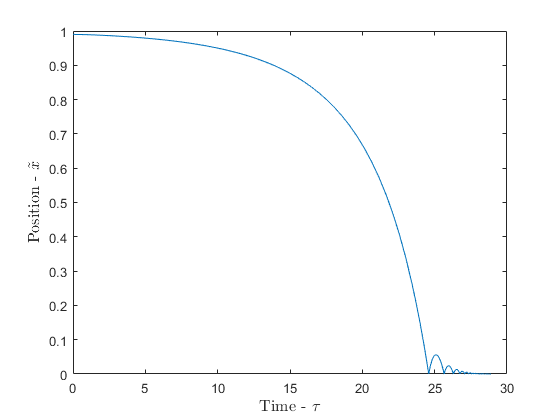
\includegraphics[width=0.7\textwidth]{Figures/Example/PositionTimeTrajectory.png}
    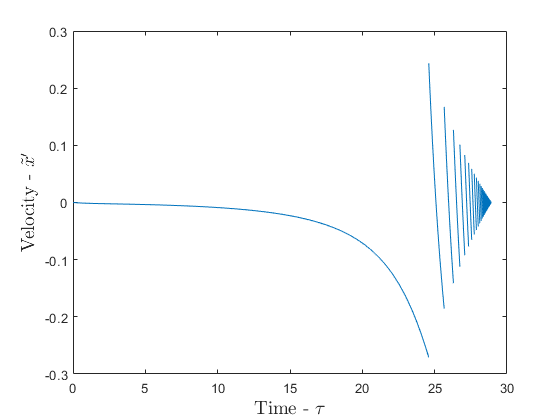
\includegraphics[width=0.49\textwidth]{Figures/Example/VelocityTimeTrajectory.png}
    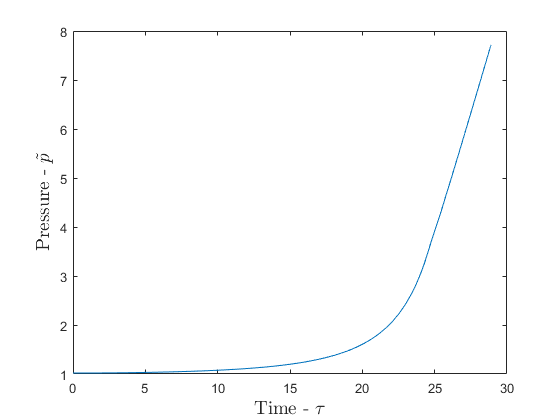
\includegraphics[width=0.49\textwidth]{Figures/Example/PressureTimeTrajectory.png}
    \caption{Simulation of \cref{eq: Non-DimODE,eq: ImpactLaw} for $\alpha = 0.1$ and $\beta = 1$. All figures are shown in the dimensionless units given by \cref{eq: BadDimensionlessVar}.}
    \label{fig:TimeTrajec}
\end{figure}

The dynamics in \cref{fig:TimeTrajec} show the desired behaviour in which the valve closes. Interestingly, the valve requires a series of impacts to gradually decrease the velocity until the valve is at rest. However, these impacts do not constitute a chatter instability, as they are low energy and non-sustained. With these impacts, the valve will close in a finite time, which will be discussed in \cref{sec: ImpactDynamics}.

\newpage
Although the valve position and velocity both tend towards zero, the tank pressure does not show similar behaviour as instead $p \rightarrow \infty$. This may initially seem slightly counter-intuitive except for two important restrictions of this simple model. Firstly, the pilot valve is completely ignored, which means the main valve will never open once it has closed as the opening mechanism is dependent on the pilot valve. Secondly, except in the limit that $\alpha \rightarrow 0$ and $\beta \rightarrow \infty$, there is also a non-zero mass flow rate into the tank, or equivalently $\dot{m}_{\rm{in}} \neq 0$. Hence, when the valve is closed, the mass of fluid is still increasing. Therefore, the density must slightly increase so the pressure must also slightly increase. \Cref{sec: ClosingFixPres} will consider an alternative approach for which the tank pressure is fixed by varying the mass flow into the tank.

% % Example Trajectory in Phase Portrait - PROBABLY NOT WORTH USING
% \begin{figure}[!ht]
%     \centering
%     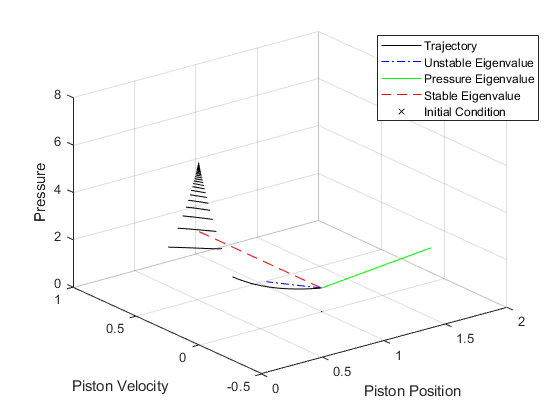
\includegraphics[width=0.49\textwidth]{Figures/Example/PhasePotrait3D.png}
%     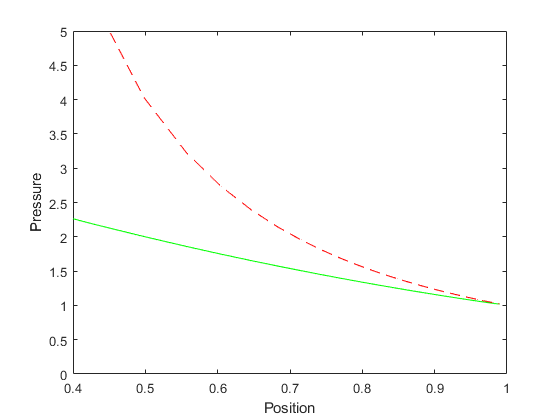
\includegraphics[width=0.49\textwidth]{Figures/Example/PressurePositionPhasePotrait2D.png}
%     \caption{Caption}
%     \label{fig:ExamplePhase}
% \end{figure}

% % Example Trajectory in eigenvector projected Phase Portrait - DO NOT USE
% \begin{figure}[!ht]
%     \centering
%     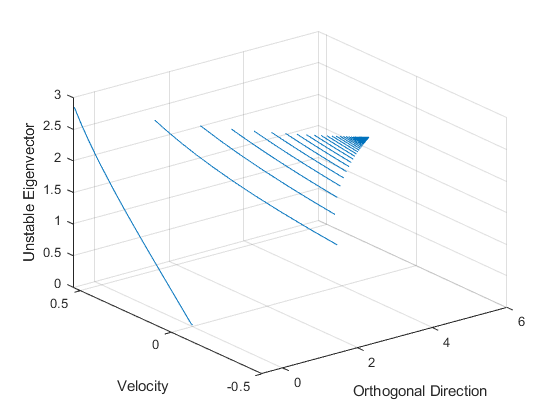
\includegraphics[width=0.7\textwidth]{Figures/Example/EigenvectorPhasePotrait3D.png}
%     \caption{Caption}
%     \label{fig:EigPhase}
% \end{figure}

% % Example Trajectory of eigenvector space in 2D Phase and 1D unstable trajectory - DO NOT USE
% \begin{figure}[!ht]
%     \centering
%     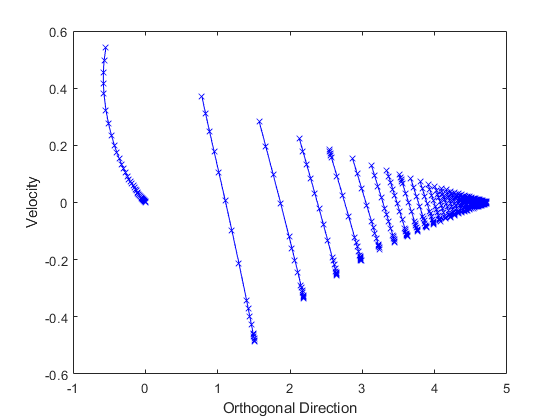
\includegraphics[width=0.49\textwidth]{Figures/Example/PhasePotrait2D.png}
%     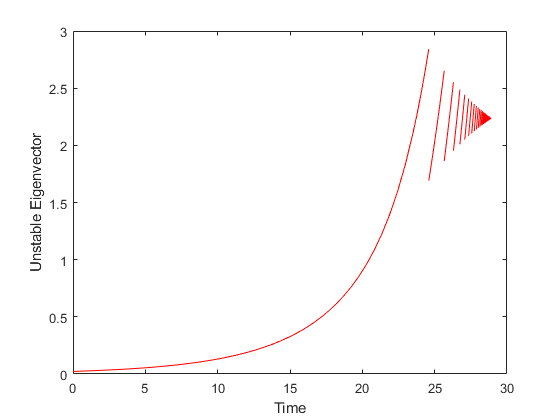
\includegraphics[width=0.49\textwidth]{Figures/Example/UnstableEigenvectorTrajectory.png}
%     \caption{Caption}
%     \label{fig:EigenvectorPhase}
% \end{figure}

\section{Low flow rate analysis}

As has been previously identified, for low flow rates where $\dot{m}_{\rm{in}} \rightarrow 0$, the limit of $\alpha \rightarrow 0$ and $\beta \rightarrow \infty$ occurs. Focusing on only the limit of $\alpha \rightarrow 0$, the eigenvalues of the linearised form of \cref{eq: Non-DimODE} around the equilibrium are
~ % eigenvalues
\begin{equation*}
    \lambda_1 = - \frac{1}{2}\beta \, , \quad
    \lambda_2 = -1 \, , \quad
    \lambda_3 = 0 \, .
\end{equation*}

Similarly, the eigenvectors in the limit of $\alpha \rightarrow 0$ are
~ % eigenvectors
\begin{equation*}
    v_1 = \begin{pmatrix}
    0 & 0 & 1
    \end{pmatrix}^T \qquad
    v_2 = \begin{pmatrix}
    \frac{2 - \beta}{2\beta} & \frac{\beta - 2}{2\beta} & 1
    \end{pmatrix}^T \qquad
    v_3 = \begin{pmatrix}
    - \frac{1}{2} & 0 & 1
    \end{pmatrix}^T \, .
\end{equation*}

This reveals several interesting results about a low flow rate scenario. Firstly, the equilibrium becomes neutrally stable. This is particularly interesting as it suggests that if there is no mass flow into the tank, the main valve will not close. However, this represents the case for which the tank equilibrium pressure is $p_t = 0$. In this case, the main piston obviously will not move as there are no fluid forces acting upon the main piston.

There is also one constant eigenvalue, $\lambda_2$, which does not depend upon $\beta$. In the limit that $\beta \rightarrow \infty$, the corresponding eigenvector is $v_2 = \left( - \frac{1}{2}, \frac{1}{2}, 1 \right)^T$. This is the only eigenvector with a component in  the velocity direction, which suggests that for sufficiently large $\beta$, the dynamics in the velocity component are near identical. \Cref{fig: ValveClose3DPhase} shows the phase portrait in position-velocity-pressure space, which shows very similar behaviour in the velocity direction for two different $\beta$ values.
~
% The three dimensional phase portrait in Position-Velocity-Pressure phase space can be seen below.
% 
\begin{figure}[ht]
    \centering
    \begin{subfigure}{0.49\textwidth}
    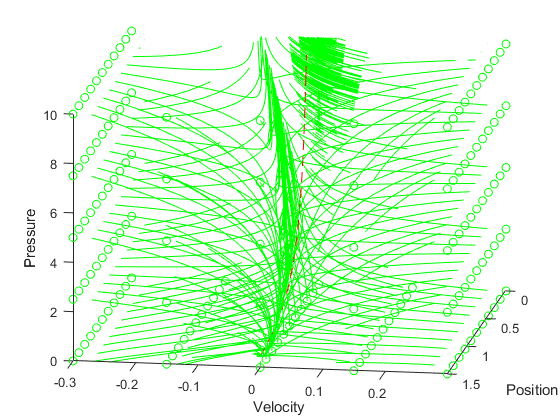
\includegraphics[width=\textwidth]{Figures/LowFlow/3DPhase-b=1.png}
    \caption{$\alpha = 0.01, \, \beta = 1$}
%    \label{fig:1}
    \end{subfigure}
    \begin{subfigure}{0.49\textwidth}
    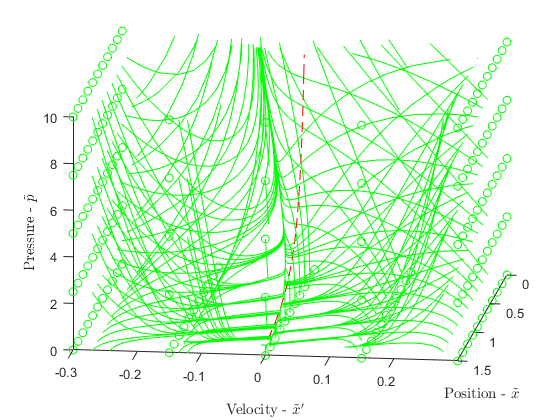
\includegraphics[width=\textwidth]{Figures/LowFlow/3DPhase-b=10.png}
    \caption{$\alpha = 0.01, \, \beta = 10$}
%    \label{fig:2}
    \end{subfigure}
    \caption{3D phase portrait of the valve closing model, \cref{eq: Non-DimODE,eq: ImpactLaw}. All details are as in \cref{fig:TimeTrajec} unless otherwise stated.}
    \label{fig: ValveClose3DPhase}
\end{figure}

\newpage
In fact, we see that the dynamics approaches the unstable manifold of the equilibrium. The valve then either follows the manifold in the direction of decreasing piston position, so that the valve closes. Alternatively, the dynamics follow the manifold with increasing valve position, so that the valve opens further to the upper stop. Regardless of the value of $\beta$ used, the unstable manifold appears to have an identical shape when projected onto the velocity-position and velocity-pressure plane. Because of this similar behaviour, phase portraits will now only show a 2D representation in the position-pressure space for clarity.

One difference which can be seen between the phase portraits for $\beta = 1$ and $\beta = 10$ (\cref{fig: ValveClose3DPhase}) is due to impact dynamics. For $\beta = 1$, the valve collides with the lower stop at a low enough pressure that it can be seen in the pressure range shown in \cref{fig: ValveClose3DPhase}. These dynamics are predictable in that an impact occurs so the velocity reverses, but the piston is still being forced downwards by the fluid. Hence, the impacts continue while the velocity tends to 0. This will be further explored in \cref{sec: ImpactDynamics}.

By looking at \cref{eq: Non-DimODE}, we see that as $\alpha \rightarrow 0$ and $\beta \rightarrow \infty$, a slow-fast system occurs. Hence, we expect the dynamics to quickly approach the equilibrium pressure, so that
~
\begin{equation*}
    1 - x \sqrt{p} = 0 \, .
\end{equation*}

This is in agreement with the eigenvalues, as $\lambda_1 \rightarrow - \infty$. The corresponding eigenvector, $v_1$, shows these dynamics purely effect the tank pressure locally to the equilibrium. In fact, this is exactly what we see in \cref{fig: ValveClose3DPhase}, where the vertical lines show the dynamics very quickly approach the equilibrium pressure. In fact, the dynamics approach the family of equilibria which exist as $\dot{m}_{\rm{in}} \rightarrow 0$. Further from the equilibrium at $\tilde{x} = 1$, the fast dynamics do not act purely horizontally.
~
% The phase portrait in Position-Pressure space can be seen below
% 
\begin{figure}[ht]
    \centering
    \begin{subfigure}{0.49\textwidth}
    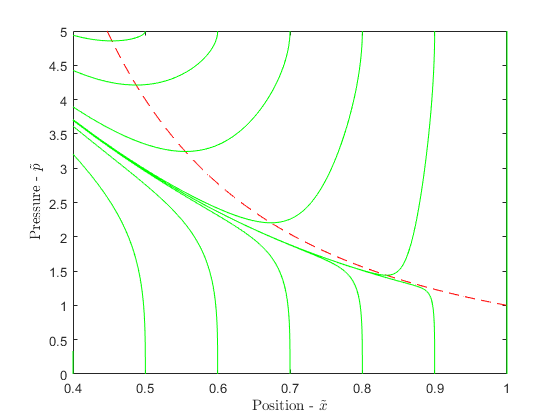
\includegraphics[width=\textwidth]{Figures/LowFlow/PhasePortrait-b=1.png}
    \caption{$\alpha = 0.01, \, \beta = 1$}
    \label{fig: ValveClosePhase1}
    \end{subfigure}
    \begin{subfigure}{0.49\textwidth}
    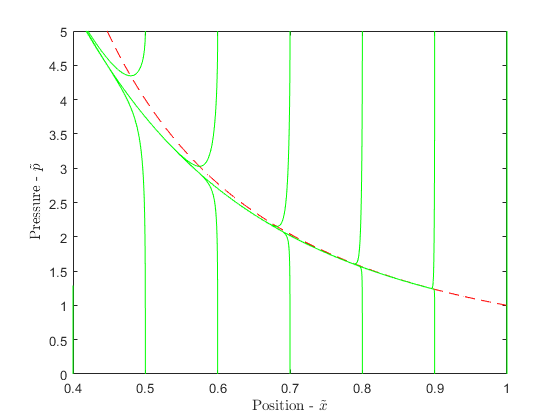
\includegraphics[width=\textwidth]{Figures/LowFlow/PhasePortrait-b=10.png}
    \caption{$\alpha = 0.01, \, \beta = 10$}
    \label{fig: ValveClosePhase10}
    \end{subfigure}
    \caption{2D representation of the phase portrait in \cref{fig: ValveClose3DPhase}}    \label{fig: ValveClosePhase}
\end{figure}

In fact, as $\alpha \rightarrow 0$ and $\beta \gg 1$, the equation $1 - \tilde{x} \sqrt{\tilde{p}} = 0$ gives a closer approximation to the unstable manifold. However, even when $\beta$ is not sufficiently large, this gives a good approximation sufficiently close to the equilibrium.
%This expression is tangeant to the unstable eigenvector given by $v_3$ at the equilibrium.

% Simulation results support this. 
% 
% % 2D Phase Portrait showing low flow rate trajectory close to manifold - PROBABLY DO NOT (TOO SIMILAR TO BELOW)
% \begin{figure}[ht]
%     \centering
%     \begin{subfigure}{0.49\textwidth}
%     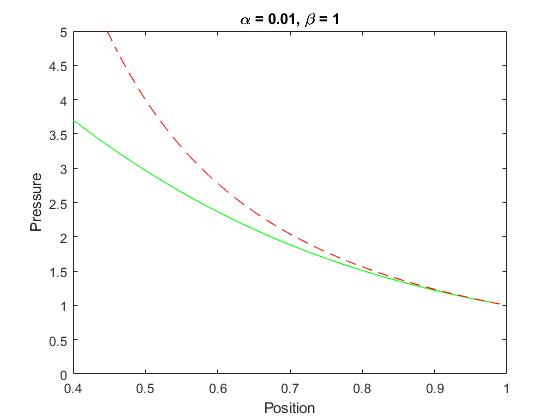
\includegraphics[width=\textwidth]{Figures/LowFlow/b=1.png}
%     \caption{$\alpha = 0.01, \, \beta = 1$}
% %    \label{fig:1}
%     \end{subfigure}
%     \begin{subfigure}{0.49\textwidth}
%     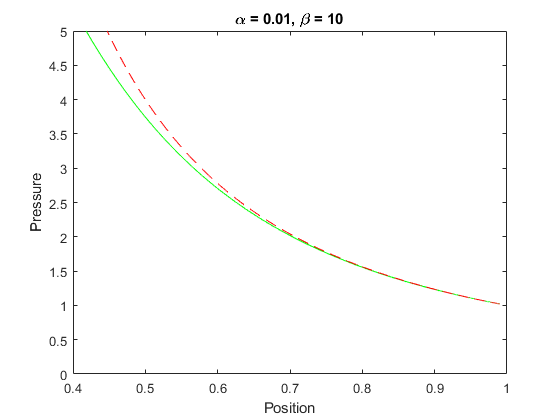
\includegraphics[width=\textwidth]{Figures/LowFlow/b=10.png}
%     \caption{$\alpha = 0.01, \, \beta = 10$}
% %    \label{fig:2}
%     \end{subfigure}
% %    \label{3}
% %    \caption{}
% \end{figure}

% \newpage
\section{Fixed tank pressure} \label{sec: ClosingFixPres}

Perhaps a more realistic case is when the mass flow rate into the tank, $\dot{m}_{\rm{in}}$, is allowed to vary such that the tank pressure remains constant. Hence, the extreme rise in tank pressure seen in \cref{fig:TimeTrajec} does not occur. As both $\alpha$ and $\beta$ are functions of $\dot{m}_{\rm{in}}$ in \cref{eq: Non-DimODE}, this set of dimensionless equations is not useful for the purpose of constant tank pressure. Instead, a new set of dimensionless equations will be introduced. These use the valve equilibrium lift as the reference distance and ambient pressure as the reference pressure.

Hence, the reference dimensions are given by
~
\begin{equation*}
\begin{split}
    x_{\rm{ref}} = \frac{1}{C_d} \sqrt{\frac{A_v - A_p}{4 \pi}}
    \, , \qquad
    p_{\rm{ref}} = p_a = 1 \, \si{bar}
    \, , \qquad
    \omega_{\rm{ref}} = C_d \sqrt{4 \pi} \sqrt{\frac{p_{\rm{ref}} x_{\rm{ref}}}{m_v}} \, .
\end{split}
\end{equation*}

Using these reference dimensions, the dimensionless set of differential equations are given by
~
\begin{equation} \label{eq: AltNonDim}
\begin{split}
    \ddash{\tilde{x}} + \kappa \, \dash{\tilde{x}} &=  \tilde{p} \left( \tilde{x}\power{2}  - 1 \right) \, , \\
    \dash{\tilde{p}} &= \beta \left( q - \sigma \mu \, \tilde{x} \, \sqrt{\tilde{p}} \right) \, .
\end{split}
\end{equation}

This system of equation uses significantly more dimensionless parameters than \cref{eq: Non-DimODE}. However, \cref{eq: AltNonDim} uses dimensionless parameters which are consistent with those used later in this report in \cref{subsec: QWMNonDim}. One important parameter is $q$, which represents the flow into the tank and is expressed in terms of the fraction of the maximum flow allowable, a fixed constant $\dot{m}_{\rm{cap}}$. The definition of all the dimensionless parameters used are
~
\begin{equation*}
    \begin{tabular}{p{2.1cm} p{2.8cm} p{2.1cm} p{3cm} p{2.8cm}}
        $ \kappa = \frac{c_v}{m_v \omega_{\rm{ref}}} \, , $
        &
        $ \beta = \frac{a^2}{V} \frac{\dot{m}_{\rm{cap}}}{p_{\rm{ref}} \omega_{\rm{ref}}} \, , $
        &
        $ q = \frac{\dot{m}_{\rm{in}}}{\dot{m}_{\rm{cap}}} \, , $
        &
        $ \mu = \frac{\rho A_p \omega_{\rm{ref}} x_{\rm{ref}}}{\dot{m}_{\rm{cap}}} \, , $
        &
        $ \sigma = \frac{\zeta x_{\rm{ref}} \sqrt{\rho p_{\rm{ref}}}}{A_p \rho x_{\rm{ref}} \omega_{\rm{ref}}} \, . $
    \end{tabular}
\end{equation*}

It is now clear why such a non-dimensionalisation was chosen. For the tank pressure to be constant, either $\beta = 0$ or the mass inflow to the tank matches that discharge through the main valve exactly. For the case that $\beta \neq 0$, the mass flow into the tank must satisfy
~
\begin{equation*}
    q = \sigma \mu \, \tilde{x} \, \sqrt{\tilde{p}} \, .
\end{equation*}

% POSSIBLY INCLUDE TWO GRAPHS OF $\tilde{x}$ AND $q$?! MAYBE SET MAXIMUM OF $q = 1$ AND SHOW PRESSURE AS VALVE CLOSING
% 
\begin{figure}[!ht]
    \centering
    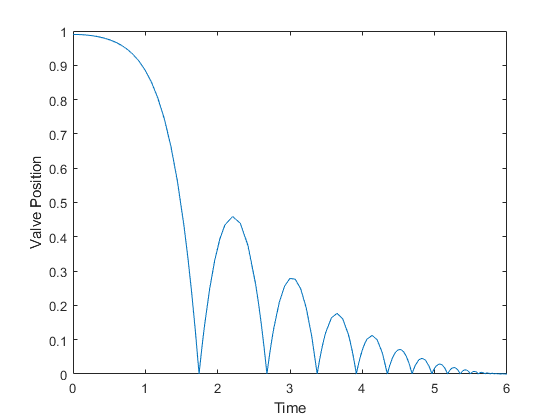
\includegraphics[width=0.49\textwidth]{Figures/FixedPressure/Position.png}
    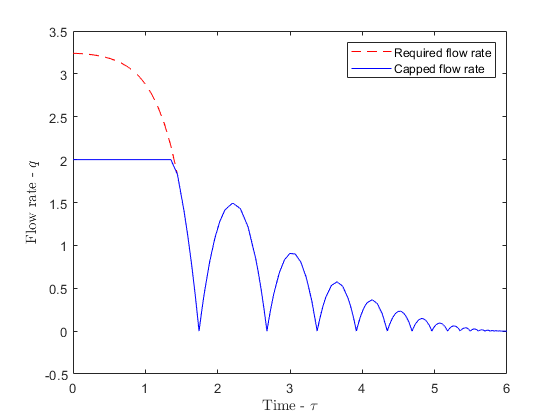
\includegraphics[width=0.49\textwidth]{Figures/FixedPressure/FlowRate.png}
    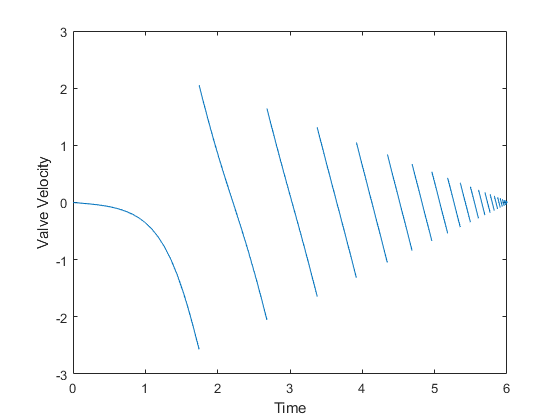
\includegraphics[width=0.49\textwidth]{Figures/FixedPressure/Velocity.png}
    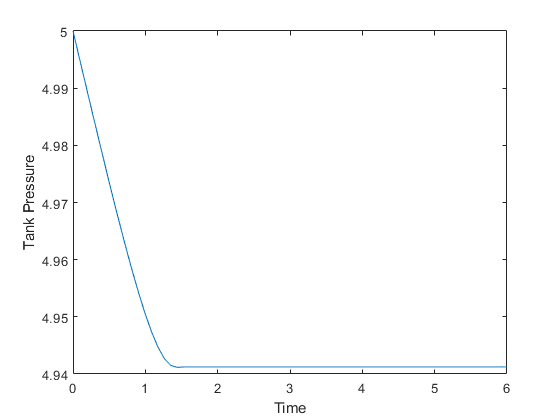
\includegraphics[width=0.49\textwidth]{Figures/FixedPressure/Pressure.png}
    \caption{Simulation of fixed tank pressure valve closing model (\cref{eq: AltNonDim}) when maximum flow rate into the tank is $q = 2$. All parameters are given in \cref{tab: ValveClosingQWMParameterValues}.}
    \label{fig: FixPres}
\end{figure}

Now, the tank pressure $\tilde{p}$ is a fixed parameter that the tank is held at. Hence, the mass flow into the tank must be directly proportional to the valve lift.

In practice, there may be a maximum flow into the tank which can be achieved. This can be modelled by using a flow rate defined by
~
\begin{equation*}
    q = \max \begin{cases} 2 & \quad \dash{\tilde{p}} \neq 0 \, , \\
    \mu \sigma \tilde{x} \tilde{p} & \quad \dash{\tilde{p}} = 0 \, .
    \end{cases}
\end{equation*}

\Cref{fig: FixPres} shows the simulation results for this case. It is clear that initially the flow rate into the tank is the maximum allowable, such that the valve is discharging more fluid than can be supplied to the tank.  Hence, the pressure is expected to decrease as is seen. However, once the valve is closed enough such that the discharge from the valve can be matched, the flow rate begins to change proportionally to the valve position. Hence, the pressure remains fixed. It can also be seen that this can be achieved even when impacts occur.

%\newpage
\section{Impact dynamics} \label{sec: ImpactDynamics}

Now some more thorough consideration of the collisions with either the upper or lower stop will be considered. This is of particular use to simulate the dynamics of the valve between the first collision with the lower stop until the valve remains fully closed. Hence, if the pilot valve dynamics are also considered, a simulation would be able to reproduce the valve closing and then re-opening which is useful to study if cycling may occur. Additionally, the same analysis may be used to accurately detect the exact time at which the pilot valve closes.

\Cref{fig: ImpactPos} shows the simulation of typical dynamics for a collision with the upper stop. The following analysis can be repeated for a collision with the lower stop, however this is almost identical so will not be considered.
~
\begin{figure}[ht]
    \centering
    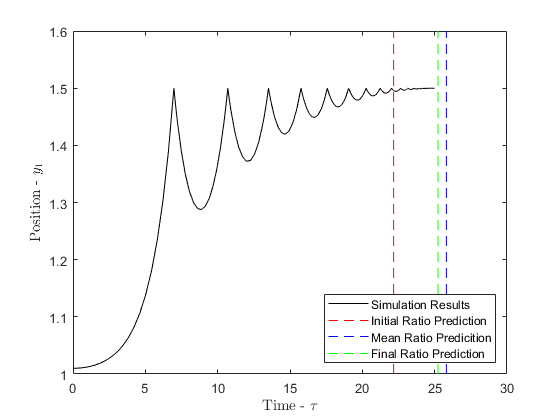
\includegraphics[width=0.7\textwidth]{Figures/ImpactSeries/PositionTime.png}
    \caption{Time trajectory of the valve position, with indications of three predictions for the final valve closing time. The red vertical dashed line (left) corresponds to using the ratio between the times of the between the first, second and third collisions. The blue vertical dashed line (right) corresponds to using the average ratio of all collisions which can be calculated. The green vertical dashed line (middle) corresponds to using the ratio between the times of the final three collisions.}
    \label{fig: ImpactPos}
\end{figure}

The important feature to notice is that the time between each successive impact seems to decrease, leading to a series of very small impacts which occur more frequently. We can consider the time between the $i$-th impact and the next impact a converging series. Hence, each term in this series may be written as
~
\begin{equation*}
    T_i = t_{i+1} - t_{i} \, ,
\end{equation*}

where $t_i$ represents the time at which the $i$-th impact occurs.

The important use of this series is to calculate the time at which the final impact occurs, at which point the valve remains closed. This is given by $t_\infty$, however this would involve an infinite number of collisions which is not feasible for simulation. Despite this, the time at which the valve remains closed, $t_f$, may be expressed as
~
\begin{equation*}
    t_f = t_\infty = t_1 + \sum^\infty_{i = 1} T_i \, .
\end{equation*}

Now we must find if the series is a geometric series for which a common ratio $r$ exists and is constant for all terms, such that $T_i = T_0 \cdot r^i$ and each successive term is the previous term multiplied by the common ratio. \Cref{fig: ImpactOtherRatio} shows how the ratio between successive terms of $T_i$ changes as more impacts occur. It can be seen that this common ratio $r$ is nearly constant over all impacts, however some small variation does exist.

If the initial common ratio, i.e. $r = \sfrac{T_2}{T_1}$, is used to predict the closing time assuming the time between collisions follows a geometric series, the time at which the valve finally closes is greatly underestimated. This can be seen in \cref{fig: ImpactPos} where the red vertical dashed line represents the time at which the valve is predicted to be fully closed. Clearly, the simulated oscillations occur past this point. This is expected from \cref{fig: ImpactOtherRatio}, where the initial common ratio is much lower than the future ratios.
~
\begin{figure}[ht]
    \centering
    \begin{subfigure}{0.49\textwidth}
    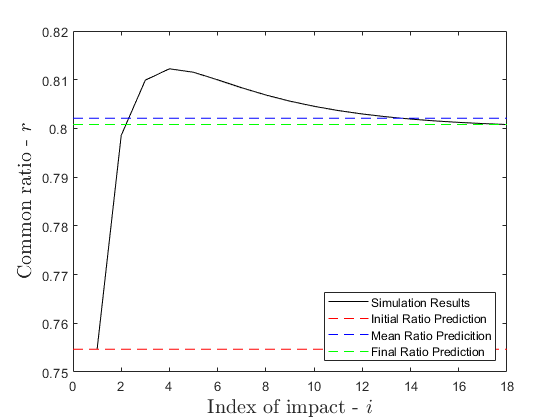
\includegraphics[width=\textwidth]{Figures/ImpactSeries/CommonRatio.png}
    \caption{Common ratio between impacts.}
    \label{fig: ImpactOtherRatio}
    \end{subfigure}
    \begin{subfigure}{0.49\textwidth}
    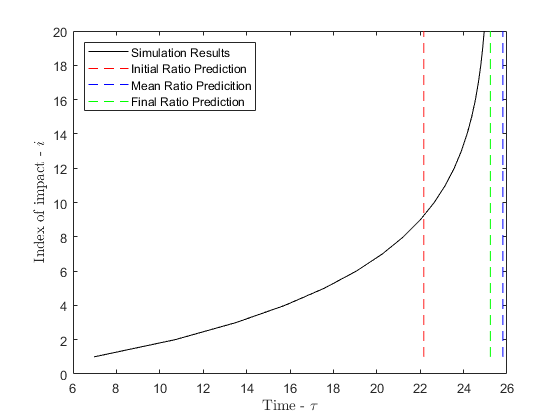
\includegraphics[width=\textwidth]{Figures/ImpactSeries/FinalTime.png}
    \caption{Time of each successive impact.}
    \label{fig: ImpactOtherTimes}
    \end{subfigure}
    \caption{Ratio between time of each impact occurring and the time of each impact.
    The red, blue and green dashed lines are coloured as in \cref{fig: ImpactPos}.
    %A red vertical dashed line (left) corresponds to using the ratio between the times of the between the first, second and third collisions. A blue vertical dashed line (right) corresponds to using the average ratio of all collisions which can be calculated. A green vertical dashed line (middle) corresponds to using the ratio between the times of the final three collisions.
    }
    \label{fig: ImpactOther}
\end{figure}

Now we consider the case for which the simulation has modelled the collisions until numerical errors prevent further simulation. It can be seen from \cref{fig: ImpactOtherRatio} that the common ratio $r$ does eventually tend towards a constant value. This means as the collisions continue to occur, the time between each impact appears to tends towards a geometric series. 

So two alternative approximations of the common ratio are used to predict the valve closing time. The first is to simply take the mean average of the common ratios. The second is to consider the geometric series only occurs continues after the collisions can no longer be simulated, such that the last calculated common ratio is used.%, such that $r = \sfrac{T_N}{T_{N-1}}$.
When these common ratios are calculated, it can be seen in \cref{fig: ImpactOtherRatio} that both give similar values for $r$.

From \Cref{fig: ImpactPos}, it is clear both of these approaches give a reasonable estimate of when the final collision occurs and the valve remains closed. However, \cref{fig: ImpactOtherTimes} shows the time at which each collision occurs. It appears using the final common ratio gives the better approximation of the finite time of the collision when $i \rightarrow \infty$. Hence, to calculate the time at which the valve remains closed, the best approximation is given by
~
\begin{equation*}
\begin{split}
    a = T_{N-2} \, , \qquad %= t_{N-1} - t_{N-2} \\
    r = \frac{T_{N-1}}{T_{N-2}} \, , \qquad %= \frac{t_N - t_{N-1}}{t_{N-1} - t_{N-2}} \\
    t_f = t_{N-2} + \frac{a}{1-r} \, ,
\end{split}
\end{equation*}

where $i = N$ is the index of the final collision which has been simulated. This may be written in terms of the time of each collision, such that

\begin{equation*}
    t_f = t_{N-2} + \frac{\left( t_{N-1} - t_{N-2} \right)^2}{2 \, t_{N-1} - t_N - t_{N-2}} \, .
\end{equation*}